\chapter{OpenStack}

OpenStack è una piattaforma di cloud computing completamente open source. Viene largamente utilizzata sia da aziende che vogliono costruirsi un proprio cloud privato che da cloud provider che offrono i loro servizi a terzi.
Una caratteristica fondamentale di OpenStack è che non è un software monolitico, ma è composto da numerosissimi componenti che permettono un'ampia personalizzazione; è possibile infatti decidere quali componenti installare in base alle funzionalità che si desiderano e su quale macchina fisica installare ciascun componente in modo che si possano costruire macchine con caratteristiche diverse in base al componente che devono ospitare (e.g. la macchina che deve contenere il componente di block storage sarà sicuramente diversa rispetto ad una che deve contendere l'hypervisor).
Oltre ai propri componenti, OpenStack utilizza anche software di terze parti, che verrà approfondito nel capitolo \ref{sec:openstack_external_components}.

\section{Componenti di OpenStack}

Di seguito verranno descritti i componenti di OpenStack che sono stati installati durante questo progetto di tesi. Esistono numerosi altri componenti che implementano altre funzionalità ma, dato che non sono stati installati o approfonditi durante lo svolgimento del progetto, non verranno trattati.

\subsection{Cinder}\label{sec:openstack_cinder}
Cinder è il servizio di block storage di OpenStack e il suo compito è quello di fornire API di block storage sia agli utenti che agli altri componenti di OpenStack. Una sua caratteristica fondamentale è che virtualizza l'accesso ai dispositivi di storage in modo che i client possano utilizzare le API che espone senza sapere quale sia il backend utilizzato. Di conseguenza Cinder non implementa al suo interno la gestione fisica dello storage ma si collega a sua volta ad altri servizi come ad esempio OpenStack Swift o Ceph (quello utilizzato in questo progetto).

\subsection{Glance}\label{sec:openstack_glance}
Glance è il servizio di immagini di OpenStack, ovvero il servizio che si occupa di scoprire, registrare e fornire le immagini di macchine virtuali e i relativi metadati. Questo componente espone una serie di API che permettono di consultare i metadati di ciascuna immagine e di prelevare le immagini stesse. Glance ha la capacità di archiviare le immagini sia su storage locale che su block storage.

\subsection{Horizon}\label{sec:openstack_horizon}
Horizon è la dashboard predefinita di OpenStack. Fornisce un'applicazione web che si interfaccia con le API di tutti i componenti installati e permette di gestire il cloud tramite un'interfaccia grafica molto più semplice e intuitiva rispetto al tool a linea di comando.

\subsection{Keystone}\label{sec:openstack_keystone}
Keystone è l'identity service di OpenStack. Si occupa di: fornire le API per l'autenticazione dei client, rilevare i servizi e implementare l'autorizzazione multi-tenant.
Supporta l'autenticazione tramite LDAP, OAuth, OpenID Connect, SAML e SQL.

\subsection{Neutron}\label{sec:openstack_neutron}
Neutron è il componente che gestisce tutta la parte di networking del cloud OpenStack. Nello specifico viene definito come un NaaS (Network as a Service) provider e permette di creare reti, sottoreti e router virtuali con lo scopo di far comunicare le macchine virtuali tra di loro con l'esterno. Gestisce anche l'assegnazione degli indirizzi IP pubblici (denominati \textit{floating IP}) e include un servizio di firewall che permette di raggruppare le regole in \textit{security groups} che poi possono essere assegnati alle macchine virtuali.

Neutron mette a disposizione una vasta scelta di plugin che permettono di scegliere quale backend utilizzare in base alle esigenze di ciascuna installazione. In questo progetto è stato utilizzato Open vSwitch perché è quello che viene consigliato di default.

\subsection{Nova}\label{sec:openstack_nova}
Nova è il componente di OpenStack che permette di creare e gestire le macchine virtuali utilizzando l'hypervisor messo a disposizione dalla macchina host. Per poter funzionare ha bisogno di interfacciarsi con i seguenti componenti di OpenStack: \hyperref[sec:openstack_keystone]{Keystone}, \hyperref[sec:openstack_glance]{Glance}, \hyperref[sec:openstack_neutron]{Neutron} e \hyperref[sec:openstack_placement]{Placement}. Nel caso in cui si voglia uno storage persistente per le macchine virtuali è richiesto anche \hyperref[sec:openstack_cinder]{Cinder}.

Nova supporta anche la gestione di server bare metal (tramite l'uso di Ironic) e ha un supporto limitato per i container, ma in questo caso specifico non abbiamo approfondito queste sue funzionalità.

\subsection{Placement}\label{sec:openstack_placement}
Placement è il componente che si occupa di inventariare e tenere traccia dei \textit{resource provider}. Un \textit{resource provider} è un pool di risorse presenti nel cloud (e.g. nodi di calcolo, storage condivisi, pool di allocazione IP).

\section{Componenti esterni a OpenStack}\label{sec:openstack_external_components}
Come accennato in precedenza, OpenStack fa uso anche di componenti di terze parti; nello specifico, quelli utilizzati in questo progetto sono: MySQL, RabbitMQ, Vault, Open Virtual Network e Ceph. Alcuni di questi sono descritti più nello specifico nei prossimi paragrafi.

\subsection{Vault}\label{sec:vault}
Vault è un sistema di gestione di \textit{secrets} e crittografia basato sull'identità. Per \textit{secret} si intende tutto ciò a cui si vuole controllare e restringere l'accesso, come ad esempio chiavi API, password, e certificati. Il compito di Vault è appunto fornire servizi di autenticazione a autorizzazione per accedere a queste risorse in maniera sicura.
\begin{figure}%[H]
    \centering
    % 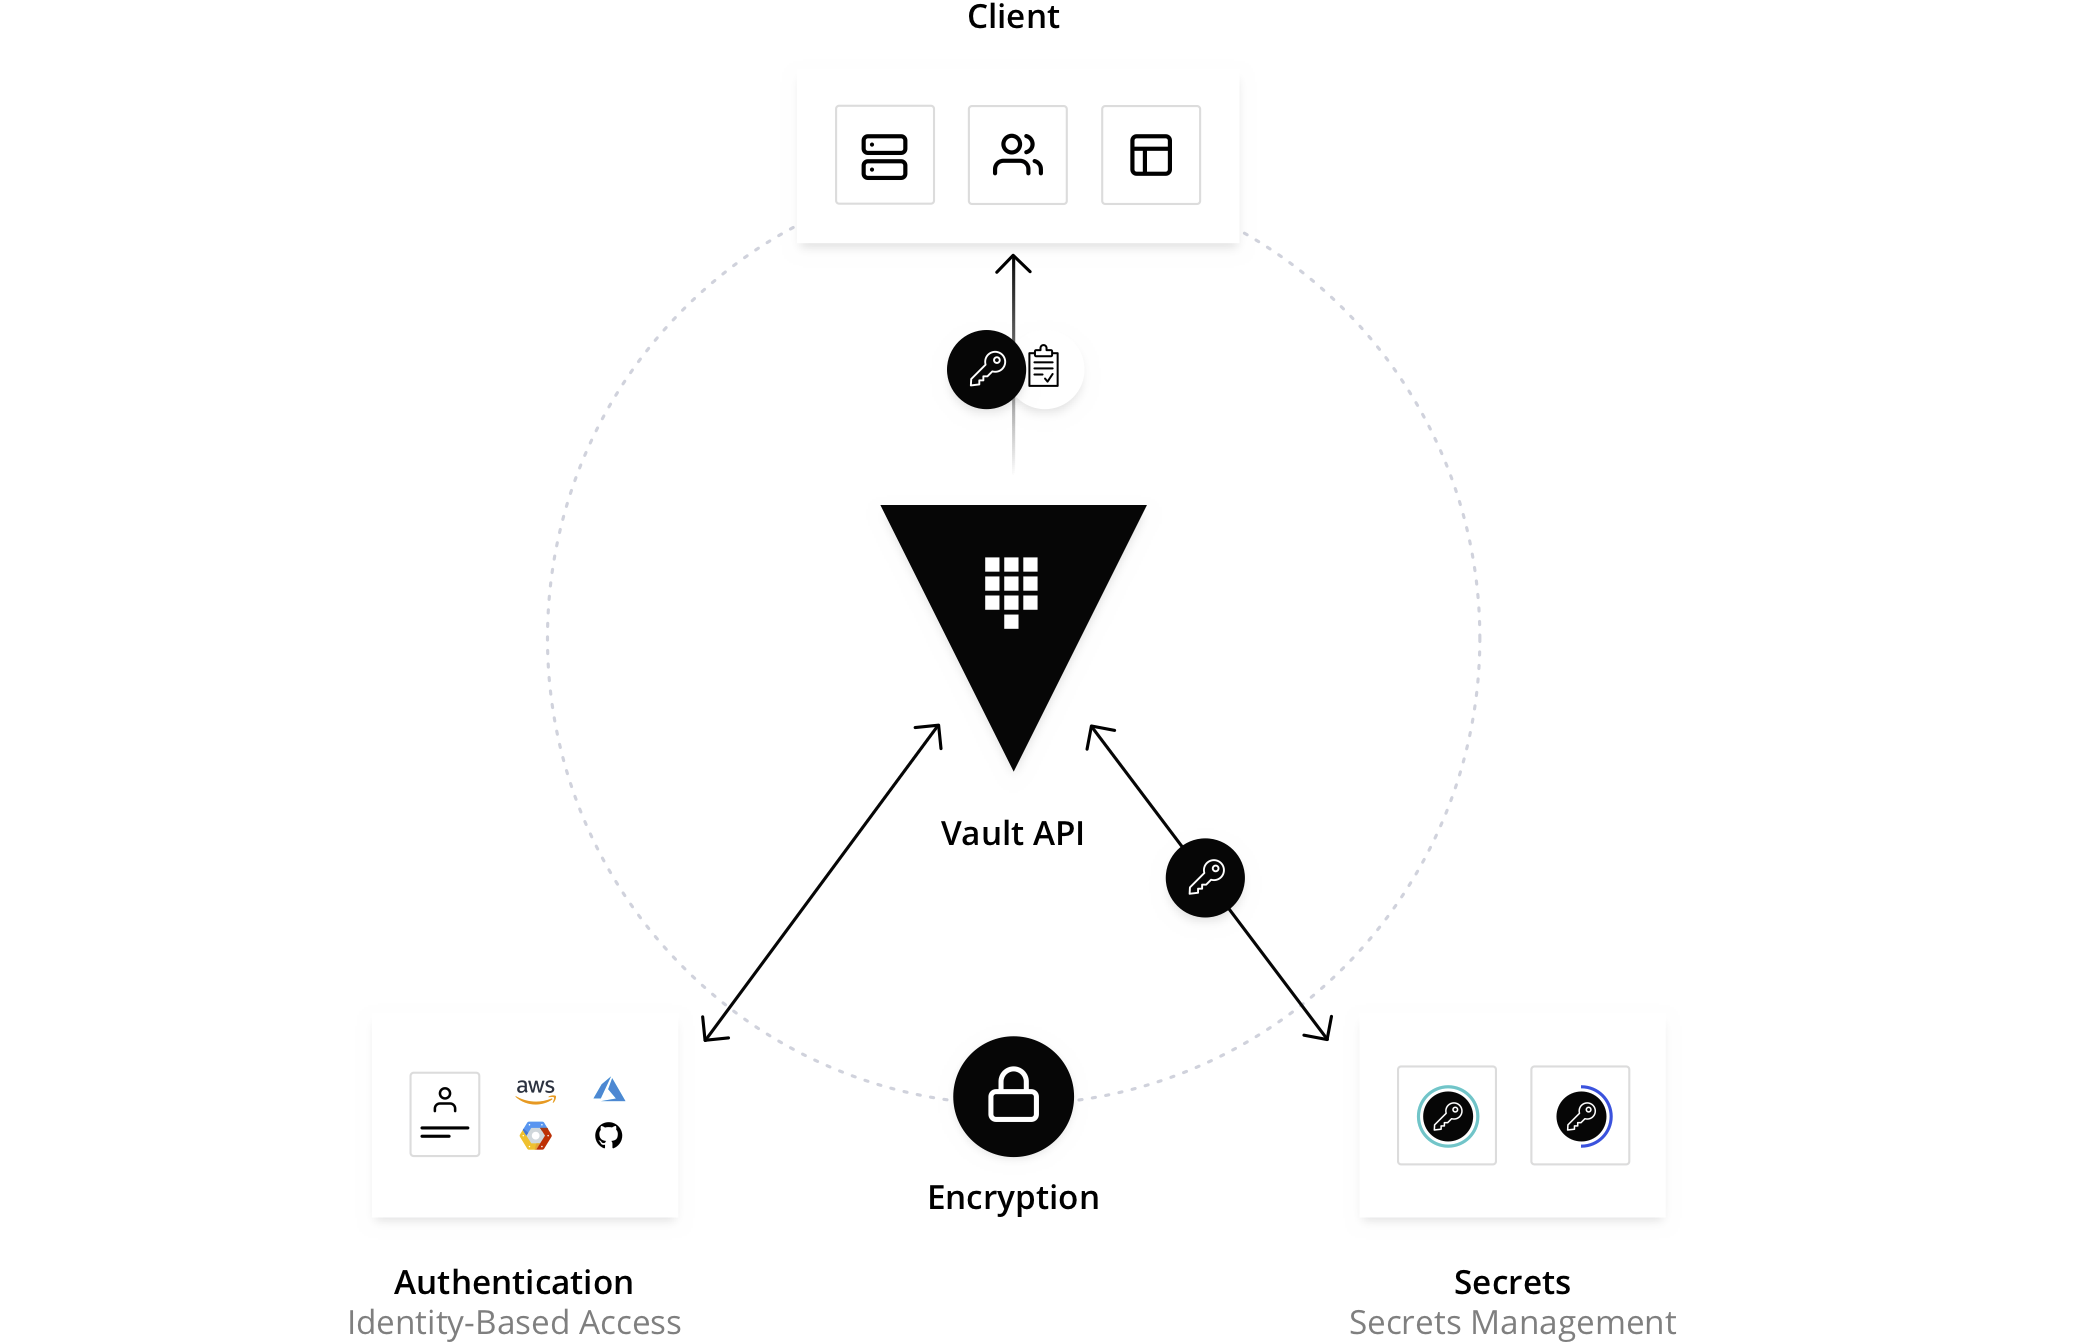
\includegraphics[scale=0.2]{tesi/files/immagini/vault_schema.png}
    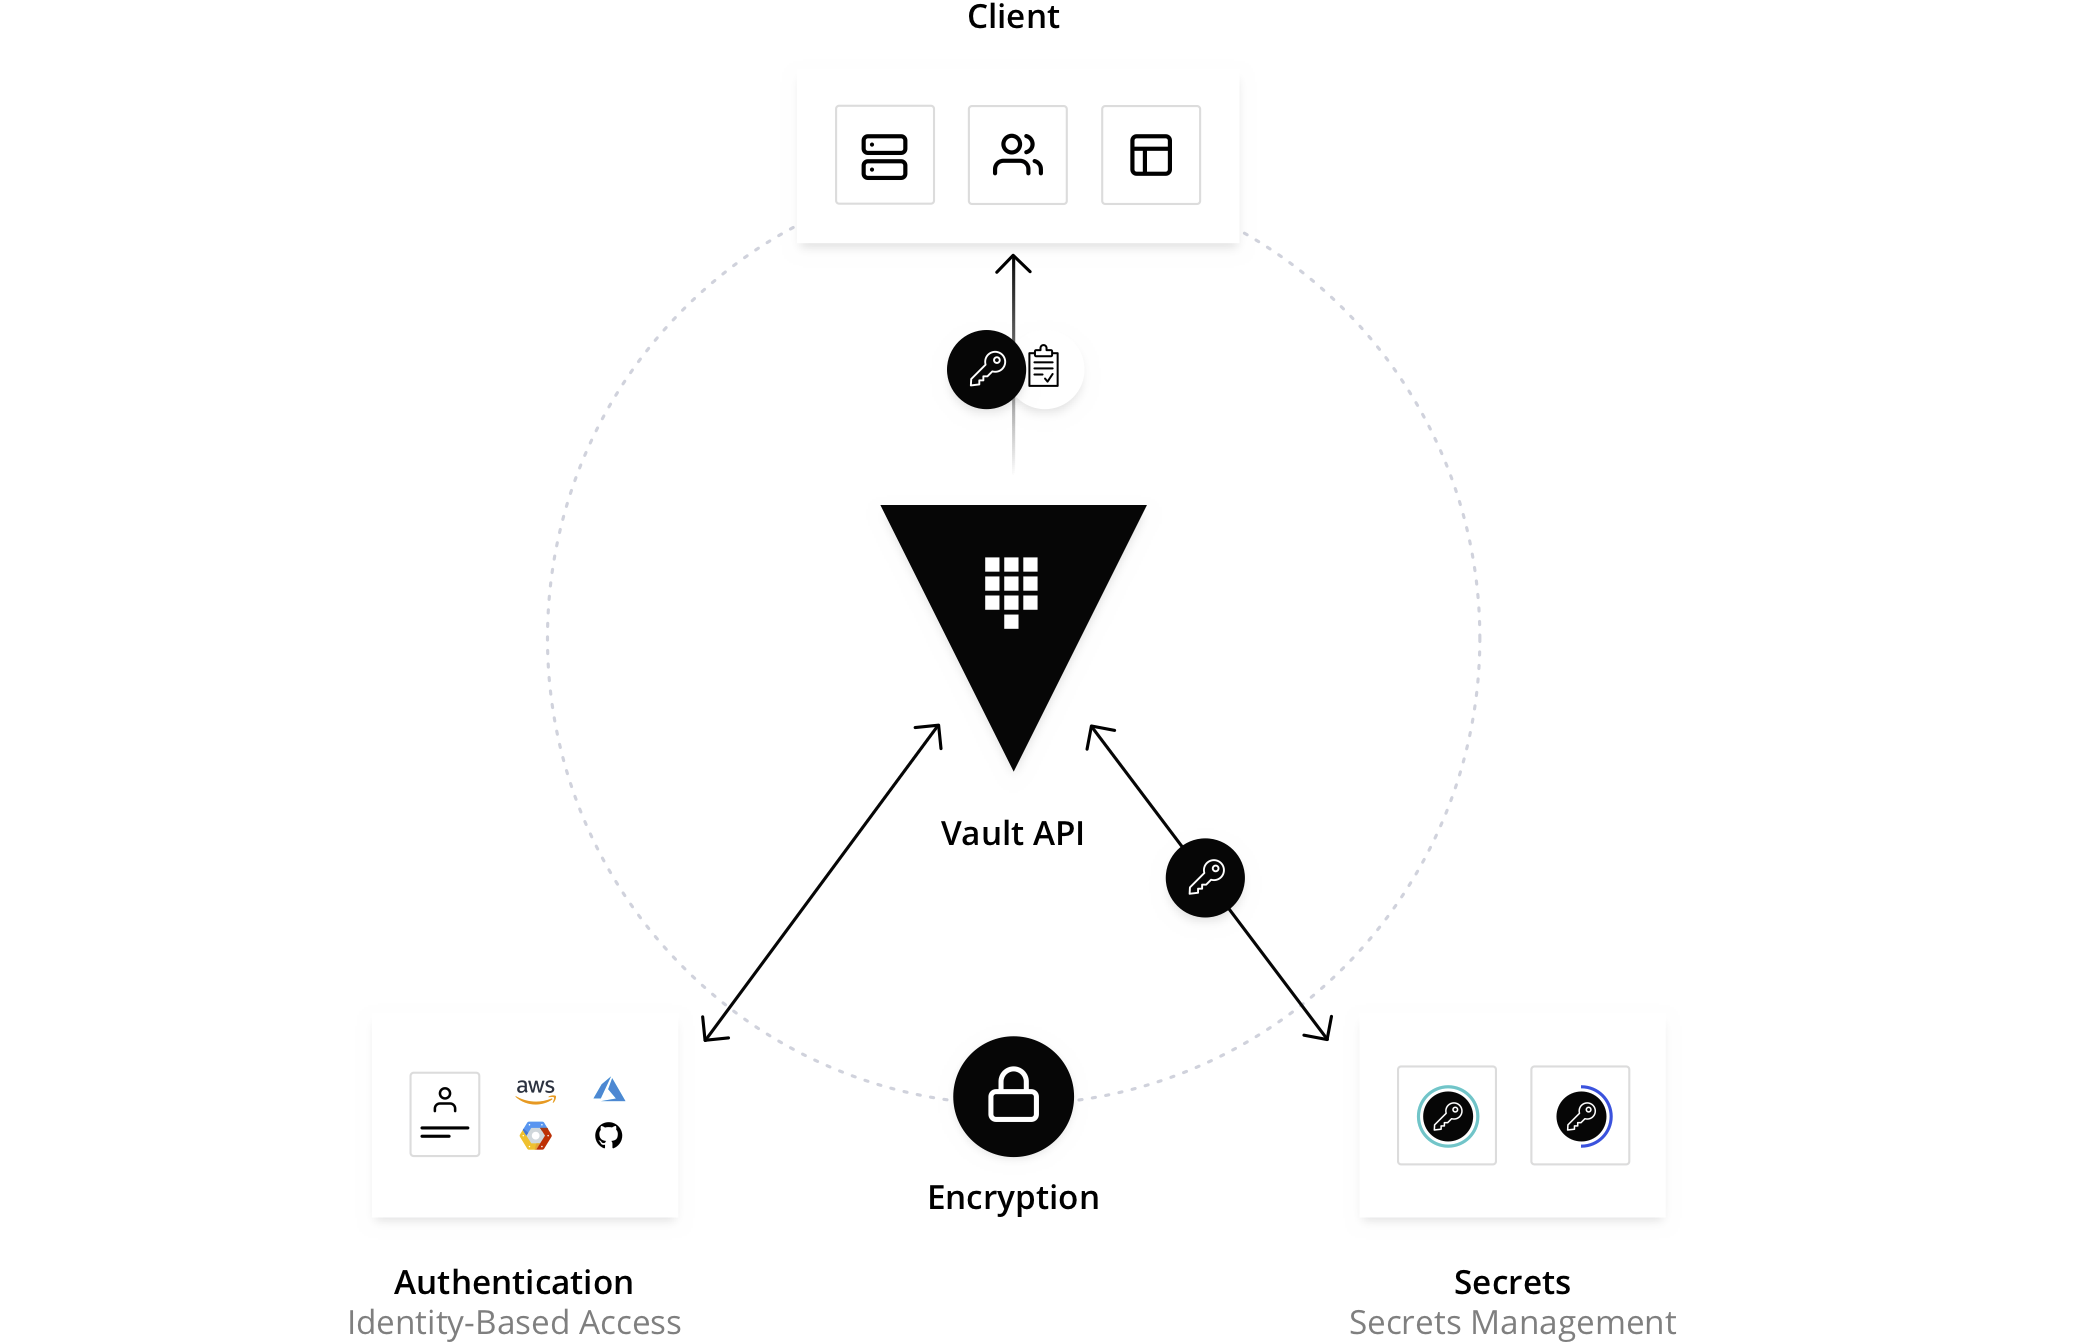
\includegraphics[width=0.9\linewidth]{tesi/files/immagini/vault_schema.png}
    %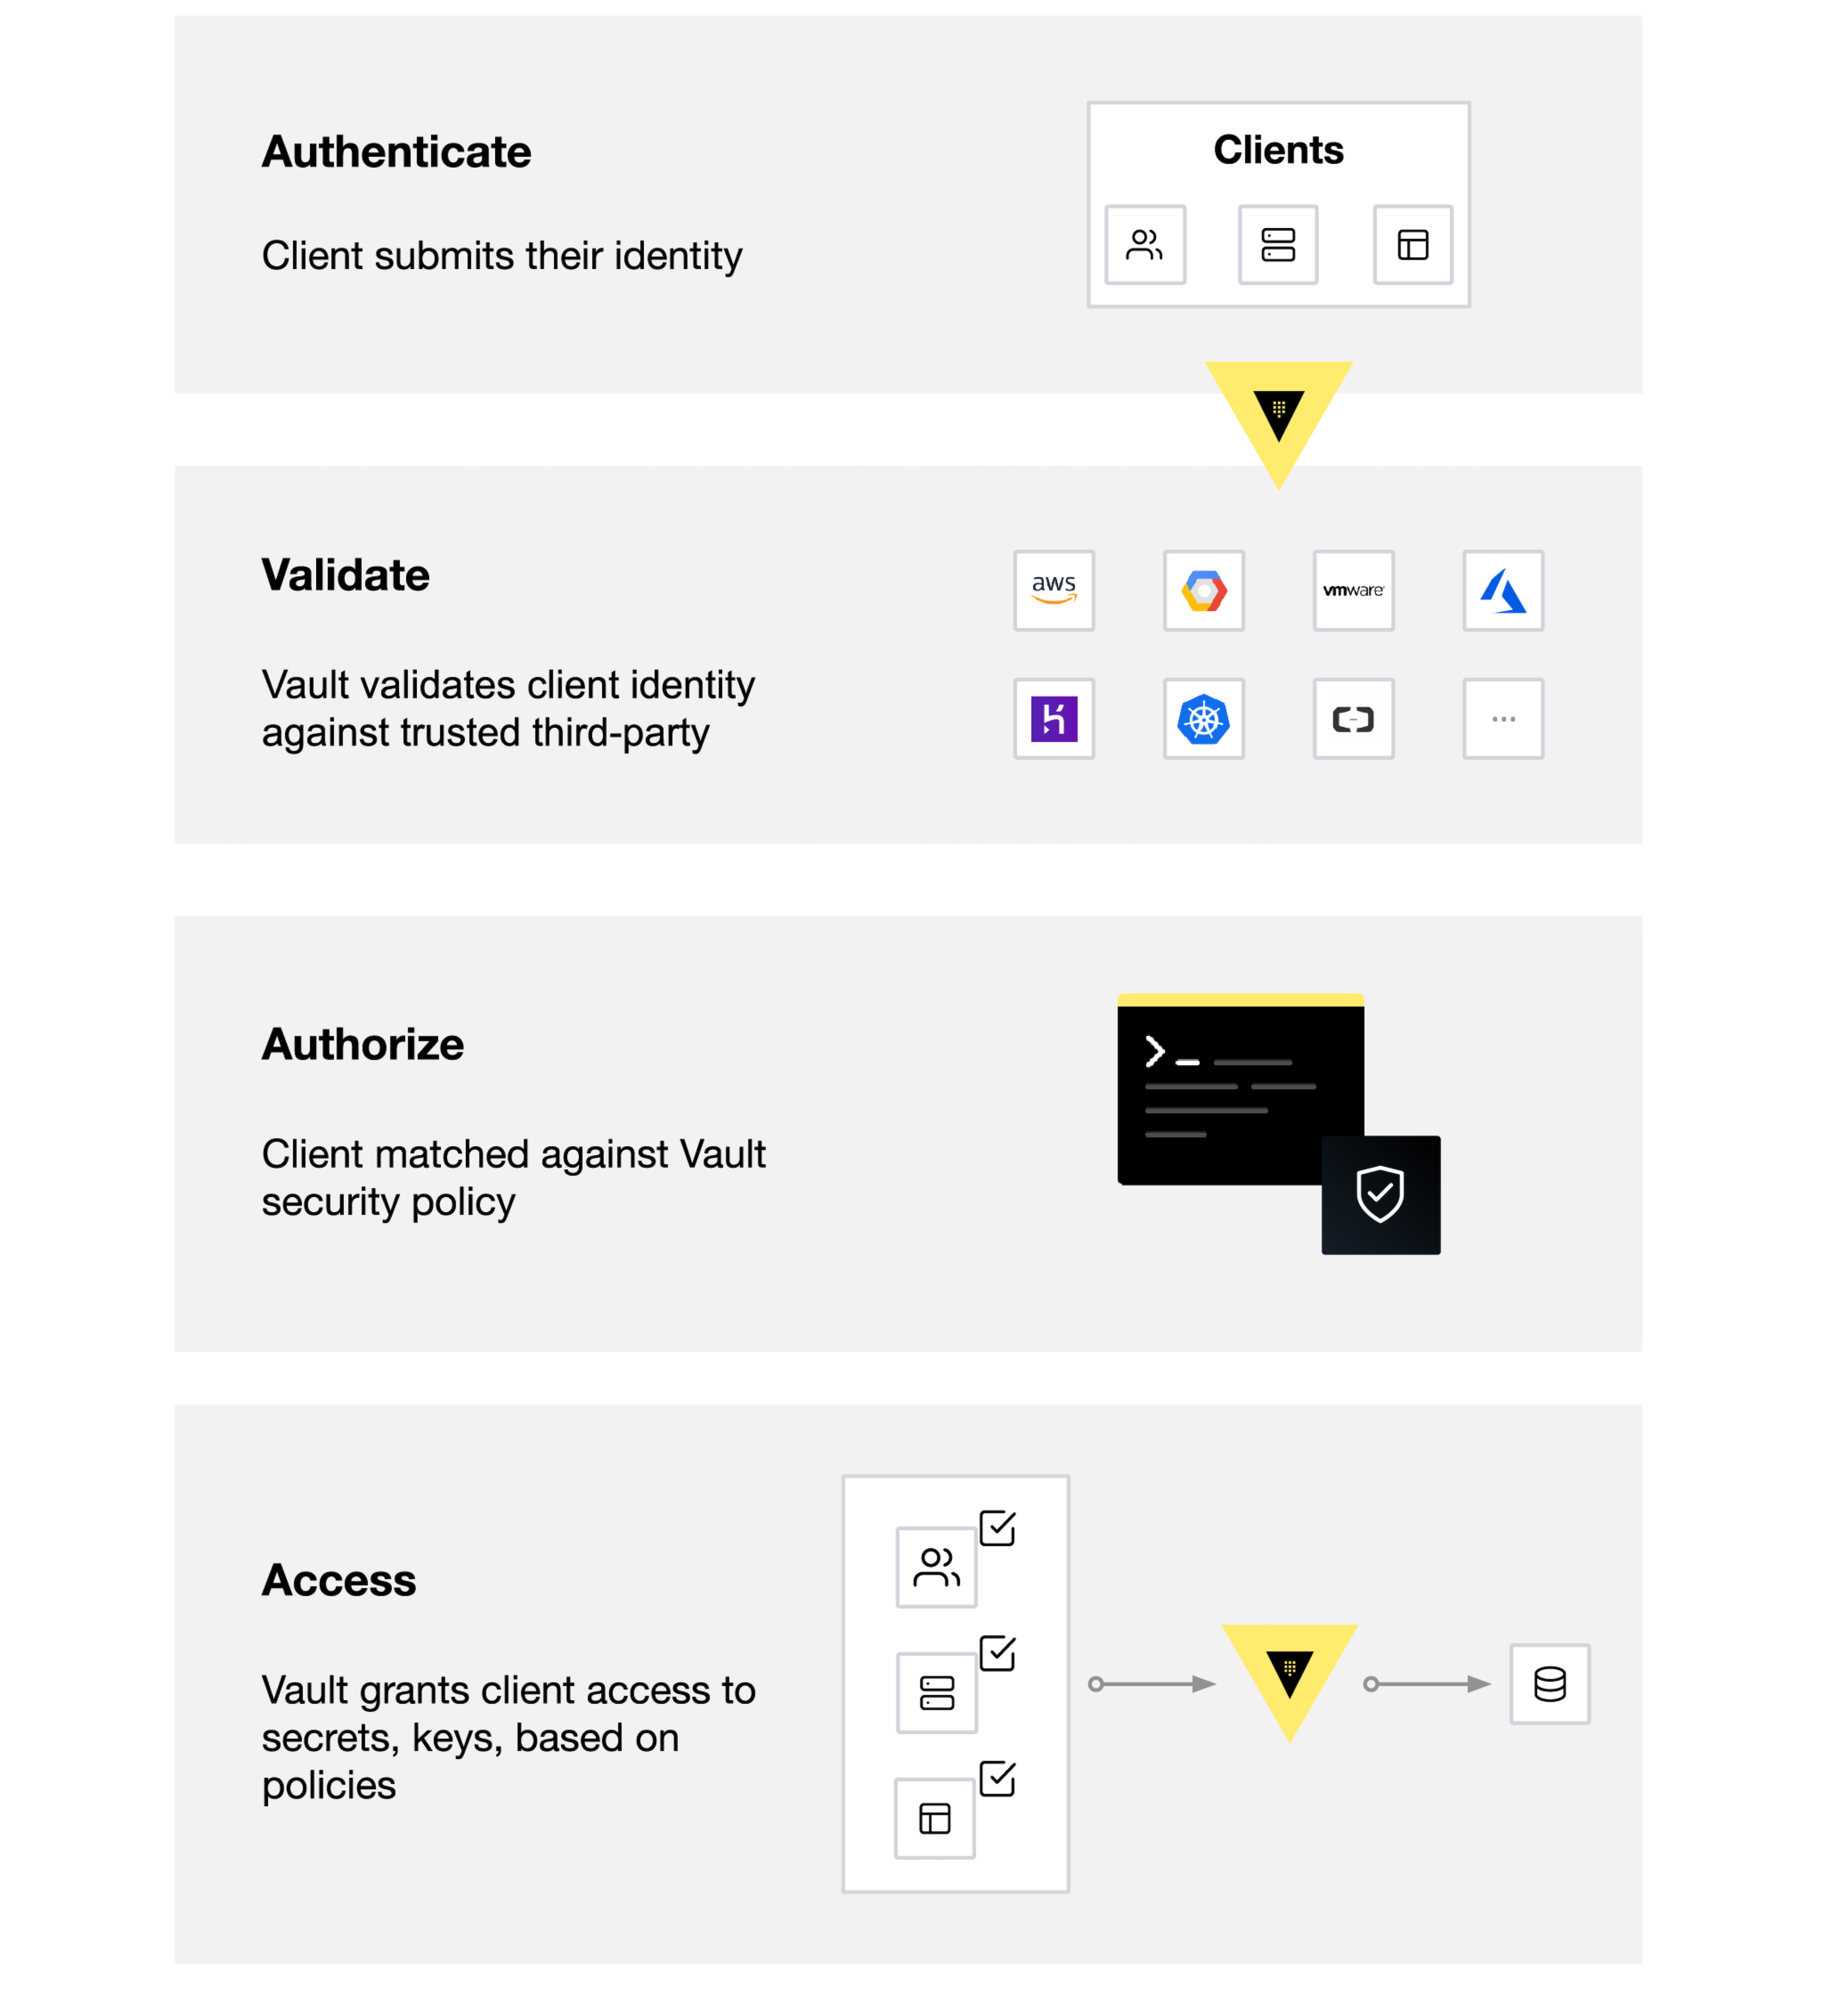
\includegraphics[scale=0.04]{tesi/files/immagini/vault_schema_2.png}
    \caption{Schema di funzionamento di Vault \cite{vault_home}.}
    \label{fig:vault_schema}
\end{figure}

In figura \ref{fig:vault_schema} è schematizzato il funzionamento di Vault. La prima cosa che ciascun client deve fare è autenticarsi e, durante questa procedura, Vault verifica l'identità attraverso il provider di autenticazione che è stato configurato. Una volta autenticato, il client può richiedere uno specifico \textit{secret} e, una volta verificato che il suddetto client abbia le autorizzazioni necessarie, Vault restituisce il \textit{secret} richiesto.

Come detto in precedenza, Vault verifica l'identità degli utenti tramite un provider di autenticazione. Sono disponibili numerosi provider che permettono di interfacciarsi con altrettanti servizi esterni (e.g. AWS, Azure, GitHub, Google Cloud, LDAP, Username e Password, ecc.), in questo modo si ha una vasta flessibilità. Il charm di Vault utilizza di default il provider basato sui Token \cite{vault_documentation}.

\subsection{Open vSwitch e Open Virtual Network}
\label{subsubsec:ovs} 

\paragraph{Open vSwitch.}Open vSwitch (OvS) è un software open source che implementa uno switch virtuale. È progettato in modo da permettere un'ampia automazione della rete mantenendo al contempo il supporto a interfacce e protocolli di gestione standard. Supporta inoltre l'installazione distribuita su più macchine fisiche \cite{ovs_home}.

\paragraph{Open Virtual Network.} Open Virtual Network (OVN) consiste in una serie di demoni che si appoggiano a Open vSwitch e implementano i layer di astrazione più alti; OVN permette infatti lavorare con router e switch logici ed è studiato per essere usato dai cloud management software (OpenStack nel nostro caso). Alcune delle sue funzionalità più rilevanti sono: router virtuali distribuiti, switch virtuali distribuiti, Access Control Lists (ACL), DHCP e DNS server \cite{ovn_home}.

\subsection{Ceph}\label{sec:ceph}
Ceph è una piattaforma open source di software-defined storage, ovvero una piattaforma software che gestisce l'archiviazione dei dati in modo indipendente dall'hardware sottostante. Una sua caratteristica fondamentale è che supporta i cosiddetti \textit{storage cluster}, che consistono nell'aggregazione di più host fisici (potenzialmente anche migliaia) in un volume di storage unico che viene poi gestito da Ceph stesso in modo che i client non debbano preoccuparsi della posizione in cui archiviare o reperire i dati \cite{ceph_documentation}.

Ciascun \textit{storage cluster} è composto da diversi componenti software:
\begin{itemize}
    \item Ceph OSD Daemon (OSD): è il demone che interagisce con i volumi di storage su ciascuna macchina che compone il cluster e si occupa dell'immagazzinamento dei dati
    \item Ceph Monitor (MON): mantiene una copia della mappa dell'intero cluster
    \item Ceph Manager: funziona insieme a Ceph Monitor e il suo compito è quello di interfacciarsi con sistemi di monitoraggio esterni (non è fondamentale per il funzionamento del cluster)
\end{itemize}

Ceph mette a disposizione 3 modalità di storage in un unico sistema: object storage, block storage e file storage.

\paragraph{Object storage.} L'object storage è un formato di storage nel quale i dati vengono archiviati in unità separate chiamati oggetti. Ciascuno di questi oggetti possiede una chiave univoca che ne permette l'individuazione all'interno di un sistema distribuito.

\paragraph{Block storage.} Il block storage è un formato di storage nel quale i dati vengono suddivisi in componenti di dimensione fissa detti blocchi, ciascuno dei quali dotato di un id univoco. Questo id, in modo analogo a quello che succede nell'obecjt storage, permette di individuare un singolo blocco all'interno di un sistema distribuito.

\paragraph{File storage.} Il file storage è il formato di storage più conosciuto: i dati vengono archiviati in una struttura gerarchica di directory. Questo è il sistema che viene utilizzato ad esempio sui computer o sui NAS \cite{storage_formats_description}.